\chapter*{Routing Fee Protocol Proposal}

Although there is methods to balance channels it would be beneficial if the fee could reflect the state in which the channel is left.

Currently the fee is only proportional to the liquidity used, not the state of the channel.

Suppose there exists a channel between Alice and Bob with 10 million satoshis in it. 
Two payments, $P_{1}$ and $P_{2}$ is routed through the channel from Bob to Alice.
Both use the same amount of liquidity 3,500,000 satoshis each, but the they start from
two different channel positions $B_{1}$ and $B_2$.

\begin{figure}[!htb]
	\hspace*{-0.7cm} 
	\centering
	\includegraphics[width=8cm]{images/protocol_upgrade.png}

	\label{fig:xt_nodes}
	\hspace*{2mm} 	
\end{figure}

The two payments would incur the same fee, 

\[ F_{P_1 P_2} = F_B + (3,500,000 * F_R / 1,000,000) \]

but leaves the channels in completely different states. $P_1$ at $B_2$ and $P_2$ at $B_4$. It is of course possible to reset the channel price after $P_1$ to
be more expensive, but suppose a third larger payment $P_3$ going from $B_1$ to $B_4$ would still run into this problem.

It is possible to limit the maximum allowed payment, to say 1/5 of the total channel capacity, so a fee could be broadcast between payments. However 
that would reduce to possible transacting parties in the network, limiting connectivity.

If the price structure was a scheme of brackets instead, where the cost depend on the channel position, these issues may be resolved. 
Each satoshi in the channel may be seen as a different bracket, with a different price for each satoshi moved. The channels would then broadcast a cost function instead of the fixed fee.

\begin{figure}[!htb]
	\vspace{-0.7cm}
	\centering
	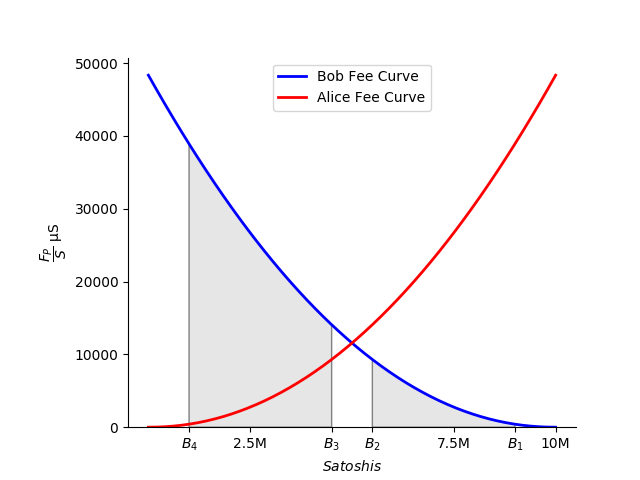
\includegraphics[width=10cm]{images/fee_scheme.png}
	\label{fig:xt_nodes}
\end{figure}
\newpage

From the cost function the fee may be retrieved by calculating the area under the graphs. Some deterministic way to round the fee to whole satoshis and some way to verify the function is formulated correctly must be defined. 

The fees for $P_1$, $P_2$ would be very different with this brackets method.

\[ F_{P_1} = F_{B} + \int_{B_1}^{B_2} f(x) dx = F_B + 13,502,153,930 \mu S \] 

\[ F_{P_2} = F_{B} + \int_{B_3}^{B_4} f(x) dx  = F_B + 88,984,850,361 \mu S \]
 
Here the fees are much larger for the payment that unbalances the channel than the payment that balances it. 

Brackets would incentivize payments to route in such a way to keep channels balanced which may lead to higher throughput. %I will most likely do a few simulations later this spring to validate this methods affect on the network.

This method has clearly some headaches accompanying it. It may be unnecessarily complex and would requires deterministic ways to calculate integrals over multiple systems. There might be better ways to solve this problem and there might be problems with this approach I'm unaware of. Anyway, some small tweaks in the protocol may lead to a much healthier network which may be worthy of exploration.\\

\textbf{John-John Markstedt}

